\documentclass{hw}

\usepackage{amssymb} %% Latex特殊符号对应表  见https://blog.csdn.net/caiandyong/article/details/53351737
\usepackage {indentfirst}  %% 中文首行缩进,需要首行缩进的段落前加上代码“\setlength{\parindent}{2em}”即可
%% 不想首行缩进, 在段落前使用命令 \noindent
\usepackage{cite}
\usepackage{natbib}   %% 引用格式问题
\setcitestyle{numbers,compress,square,comma,super}
%\usepackage[sectionbib]{chapterbib} %% 分章节参考文献
\usepackage[hyperfootnotes=false]{hyperref}
\hypersetup{
  colorlinks,
  citecolor=red,
  linkcolor=blue,
  urlcolor=blue,
 % citebordercolor=Violet,
 % filebordercolor=Red,
 % linkbordercolor=Blue
}
\usepackage{color} %% 批注颜色设置 \color{blue}这一排的字体是蓝色。 或者 \textcolor[rgb]{1,0,0}{text}
\usepackage[d]{esvect} %% 矢量箭头 见https://mirrors.bfsu.edu.cn/CTAN/macros/latex/contrib/esvect/esvect.pdf
\usepackage{tabularray} %% 表格的使用(P46有关于diagbox的说明)https://mirrors.ustc.edu.cn/CTAN/macros/latex/contrib/tabularray/tabularray.pdf 非常Nice
\UseTblrLibrary{diagbox}
\UseTblrLibrary{booktabs}
%% 嵌入MATLAB代码块 见https://mirrors.ustc.edu.cn/CTAN/macros/latex/contrib/matlab-prettifier/matlab-prettifier.pdf,也可参考以下https://zhuanlan.zhihu.com/p/388676497
\usepackage{listings}
\usepackage{xcolor}
\usepackage{textcomp}
\usepackage{matlab-prettifier}
%% 使用时只需要添加以下代码即可:\lstinputlisting[style=Matlab-editor,basicstyle=\mlttfamily,numbers=left,frame=single,caption={\bf main.m}]{L3/sample.m}
\usepackage{graphicx}
\usepackage{ragged2e} %% 首行缩进
\usepackage{float} %% 图片位置固定
%% 关键信息高亮 见https://latex-tutorial.com/color-latex/
\usepackage[dvipsnames]{xcolor}
\usepackage{soul}
\usepackage{xcolor}
%% 斜分数 \nicefrac{}{}
\usepackage{units}
\usepackage{makecell}


\course
{纳米光子学及其应用}
{Fall 2022}
{UESTC}

\assignment
{第二次作业}
{11个思考题}

\student
{张豪}
{202221050516}
{Z\_Howe94@163.com}

\begin{document}
%\sethlcolor {Aquamarine} %% 高亮颜色 使用方式:\hl{Englishtext} 或 \hl{\mbox{中文text}}

\newproblemset{problem}{思考}{思考题}
\newproblemset{computerexercise}{Computer Exercise}{Computer Exercises}
\newcommand{\pll}{\kern 0.56em/\kern -0.8em /\kern 0.56em}
\maketitle

\makeproblem

\begin{problem} % 1
什么是近场和远场?近场和远场各具有什么特点?
\end{problem}

\justifying{\setlength{\parindent}{0em}{Answer:}


\justifying{\setlength{\parindent}{2em}{近场指的是从物体表面到一个波长以内距离的电磁场,而远场指的是从近场以外一直延伸到无穷远区域的电磁场。}

\justifying{\setlength{\parindent}{2em}{波在近场中是被局域化的,且结构具有较小的空间尺度,不向外辐射能量,但可以通过相互作用传递能量,近场具有更大的波矢分量,即有$k_x>k$,可以用来探测精细的结构信息;}

\justifying{\setlength{\parindent}{2em}{波在远场中是辐射化的,且结构具有较大的空间尺度,在真空中能无损失地辐射能量,远场具有较小的波矢分量,即有$k_x<k$,可以用来探测粗略的结构信息。}

%\[
%-\dfrac{\hbar^2}{2m}\dfrac{d^2}{dz^2}\psi(z)+U(z)\psi(z)=E\psi(z)
%\]
%
%\justifying{\setlength{\parindent}{2em}{$E$为电子沿$z$方向运动的能量,而限制电子运动的势能函数$U(z)$可以表示为}
%\begin{equation}
%	U(z) =
%	\begin{cases}
%		0, & (-L_z/2<z<L_z/2) \\
%		\infty, & (z<-L_z/2,z>L_z/2)}
%	\end{cases}
%	\label{eq11}
%\end{equation}
%
%\justifying{\setlength{\parindent}{0em}{由于势垒无限高,电子不能逸出势阱,即在$z=\pm L_z/2$处波函数$\psi(z)$必须是0。利用这一条件可以得出,电子沿$z$方向运动的能量只能取下述的分立值:}
%\[
%E_{nc}=\dfrac{(\pi\hbar)^2}{2m_e^*}(\dfrac{n}{L_z})^2 \qquad n=1,2,3,\cdots
%\]
%
%\justifying{\setlength{\parindent}{0em}{相应的波函数为}
%\begin{equation}
%	\psi_n(z) =
%	\begin{cases}
%		\cos (n\dfrac{\pi}{L_z}z), & n=1,3,5,\cdots \vspace{1em} \\
%		\sin (n\dfrac{\pi}{L_z}z), & n=2,4,6,\cdots
%	\end{cases}
%	\label{eq12}
%\end{equation}
%
%\justifying{\setlength{\parindent}{0em}{另一方面,电子在$x-y$平面内自由运动,能量连续变化,}
%\[
%E_{xy}=\dfrac{\hbar^2}{2m_e^*}(k_x^2+k_y^2)=\dfrac{\hbar^2k_\perp^2}{2m_e^*}
%\]
%
%\justifying{\setlength{\parindent}{0em}{$k_x$和$k_y$分别为$x$方向和$y$方向的电子波矢。所以,电子在势阱中运动的总能量为}
%\[
%E_c(k\prep,n)=\dfrac{\hbar^2k_\perp^2}{2m_e^*}+\dfrac{(\pi\hbar)^2}{2m_e^*}(\dfrac{n}{L_z})^2 \qquad n=1,2,3,\cdots
%\]
%
%\justifying{\setlength{\parindent}{2em}{不妨取$n=1$和$n=2$,其能量间隔为:}
%\[
%\Delta E=\dfrac{(\pi\hbar)^2}{2m_e^*}(\dfrac{2}{L_z})^2-\dfrac{(\pi\hbar)^2}{2m_e^*}(\dfrac{1}{L_z})^2=\dfrac{(\pi\hbar)^2}{2m_e^*}\dfrac{3}{L_z^2}
%\]
%\justifying{\setlength{\parindent}{0em}{对于电子的德布罗意波长满足下式:}
%\[
%\dfrac{1}{2m_e^*}=\dfrac{\lambda_e^2}{h^2}k_BT
%\]
%\justifying{\setlength{\parindent}{0em}{代入能量间隔表达式,可以简化为:}
%\[
%\Delta E=\dfrac{3}{4}(\dfrac{\lambda_e}{L_z})^2k_BT
%\]
%\justifying{\setlength{\parindent}{0em}{由上式可以看出,相邻能级之间的能量间隔与$k_BT$有关。当物体尺寸$L_z\gg\lambda_e$时,能级间距越来越小,可以看做连续能级,此时给予电子一定的热激发,电子几乎可以在各个能级之间运动,那么也就不能有“能级”一说了;而当物体尺寸与电子的德布罗意波长相当或者$L_z\ll\lambda_e$时,能级间距越来越大($>k_BT$),可以看做离散能级,此时,只有输入能量$\sim k_BT$时才能激发电子进行能级跃迁,即量子效应愈发显著。}
\end{answer*}

\begin{problem} % 2
为什么利用近场可以探测超越分辨率极限的精细结构信息?
\end{problem}

\justifying{\setlength{\parindent}{0em}{Answer:}

\justifying{\setlength{\parindent}{2em}{根据测不准原理可知,若波矢分量大于其模量,则可以突破衍射极限,即$\Delta x<\lambda/2$。因此问题变为了为什么近场具有波矢分量大于其模量的特点。}

\justifying{\setlength{\parindent}{2em}{假定物体表面为$x-y$平面$(z=0)$,位于$(x,y)$处的光场可以表示为:}
\begin{equation}
E(x,y,0)=\dfrac{1}{2\pi}\iint U_0(k_x,k_y)e^{i(k_xx+k_yy)}dk_xdk_y
\label{eq1}
\end{equation}

\justifying{\setlength{\parindent}{0em}{由亥姆赫兹方程$\nabla^2E+k^2E=0$,可以得到在$(x,y,z)$处的角谱为:}
\begin{equation}
U(k_x,k_y,z)=U_0(k_x,k_y)\exp(iz\sqrt{k^2-k_x^2-k_y^2})=U_0(k_x,k_y)e^{ik_zz}
\label{eq2}
\end{equation}

\justifying{\setlength{\parindent}{0em}{当$k_x^2+k_y^2>k^2,k_z=i\kappa$时,式(\ref{eq2})为:}
\begin{equation}
U(k_x,k_y,z)=U_0(k_x,k_y)e^{-\kappa z}
\label{eq3}
\end{equation}

\justifying{\setlength{\parindent}{0em}{场在$z$方向衰减,故为局限于表面的隐失场(即近场)。假定物体表面为一系列不同周期光栅的叠加,则衍射光波矢分量($a$、$b$为可能的$x$、$y$方向的光栅周期)有:}
\begin{equation}
k_x=\dfrac{2n\pi}{a},k_y=\dfrac{2m\pi}{b},n,m=1,2,3...
\label{eq4}
\end{equation}

\justifying{\setlength{\parindent}{0em}{如果$a,b<\lambda$,则$k_x,k_y>k$对应隐失场,即小于波长的精细结构对应隐失场,不能传播到远处,故利用近场可以探测超越分辨率极限的精细结构信息。}

%\fcolorbox{white}{green}{\mbox{1、弱限制}}
%
%\justifying{\setlength{\parindent}{2em}{假定我们的纳米晶为球形,其半径为$a$,且满足$a\gg a_B^{*}$时,其中$a_B^{*}$为激子玻尔半径。这种情况我们称之为弱限制。此时,激子的能量可以表示为:}
%\[
%E_{nml}=E_g-\dfrac{\text{Ry}^*}{n^2}+\dfrac{\hbar^2\chi_{ml}^2}{2Ma^2},\qquad n,m,l=1,2,3,...	
%\]
%
%\justifying{\setlength{\parindent}{2em}{其中,$\chi_{ml}$为贝塞尔函数的根,如表1所示。$M=m_e^*+m_h^*$为激子质量,等于电子有效质量$m_e^*$和空穴有效质量$m_h^*$之和。}
%\begin{table}[H]
%    \centering
%    \fontsize{8}{10}\selectfont    %{字体尺寸}{行距}
%    \caption{贝塞尔函数$\chi_{nl}$的根}
%	\begin{tblr}{
%        row{odd} = {bg=azure8},
%        row{1} = {bg=azure3, fg=white},
%        colspec={c|ccc},
%        }
%	    \toprule
%		$l$ & $n=1$ & $n=2$ & $n=3$ \\
%	    \specialrule{0.5pt}{4pt}{6pt}
%		0 & 3.142(\pi) & 6.283(2\pi) & 9.425(3\pi)\\
%        1 & 4.493 & 7.725 & 10.904\\
%        2 & 5.764 & 9.095 & 12.323\\
%        3 & 6.988 & 10.417 &  \\
%        4 & 8.183 & 11.705 &  \\
%        5 & 9.356 &   &  \\
%        6 & 10.513 &   &  \\
%        7 & 11.657 &   &  \\
%	    \bottomrule 
%	\end{tblr}
%   % \label{tab:1}
%\end{table}
%
%\fcolorbox{white}{green}{\mbox{2、强限制}}
%
%\justifying{\setlength{\parindent}{2em}{假定我们的纳米晶为球形,其半径为$a$,且满足$a\ll a_B^{*}$时,其中$a_B^{*}$为激子玻尔半径。这种情况我们称之为强限制。此时,对于最低能级$1s1s$态,激子能量可以表示为:}
%\[
%E_{\text{1s1s}}=E_g+\pi^2(\dfrac{a_B^*}{a})^2\text{Ry}^*-1.786\dfrac{a_B^*}{a}\text{Ry}^*-0.248\text{Ry}^*	
%\]
%
%\justifying{\setlength{\parindent}{2em}{强限制可以使半导体量子点的光吸收边大于带隙宽度,对于理想量子点而言(如下图所示),强限制使得原本连续的吸收谱(吸收峰在禁带)离散化,此时的多个吸收峰均高于禁带。}
%
%\begin{figure}[H]
%\centering
%	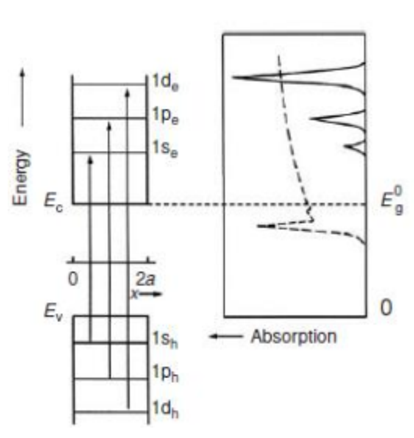
\includegraphics[width=0.4\textwidth]{L3/f9.pdf}
%\caption{\justifying{理想量子点能级与吸收谱}}
%\label{f10}
%\end{figure}
%
%\end{answer*}

\begin{problem} % 3
原子力显微镜(AFM)有几种工作模式?各模式的优、缺点是什么?
\end{problem}

\justifying{\setlength{\parindent}{0em}{Answer:}

\justifying{\setlength{\parindent}{2em}{原子力显微镜(AFM)有三种工作模式,分别为接触模式,非接触模式和轻敲模式。这三种模式各自的优缺点如下表(\ref{tab1})所示。}
\begin{table}[H]
    \centering
    \fontsize{8}{10}\selectfont    %{字体尺寸}{行距}
    \caption{AFM三种模式的优缺点}
	\begin{tblr}{
        row{odd} = {bg=azure8},
        row{1} = {bg=azure3, fg=white},
        colspec={c|cc},
        }
	    \toprule
		工作模式 & 优点 & 缺点 \\
	    \specialrule{0.5pt}{4pt}{6pt}
		接触 & \makecell[c]{快速扫描、适用于与较粗糙坚硬样品\\摩擦力分析,可在液体中扫描} & \makecell[c]{摩擦力会损害或改变表面形貌\\特别是柔软的表面}\\
        非接触 & \mbox{不损坏样品和尖端} & \mbox{分辨率低,受环境影响大} \\
        轻敲 & \makecell[c]{适用于表面容易受损、表面松弛的样品\\特别是生物样品} & \mbox{扫描速度慢,难以在溶液中扫描} \\
	    \bottomrule 
	\end{tblr}
    \label{tab1}
\end{table}

%\justifying{\setlength{\parindent}{2em}{式(\ref{eq:a3})中的$\gamma$为阻尼频率。通过求解该运动方程,可以求出金属的介电常数为:}
%\begin{equation}
%\epsilon(\omega)=1-\dfrac{\omega_p^2}{\omega^2+i\omega\gamma},\qquad \omega_p=\sqrt{\dfrac{Ne^2}{\varepsilon_0m}}
%\label{eq:4}
%\end{equation}
%\justifying{\setlength{\parindent}{2em}{其中,$\omega_p$为体积等离子体激元的固有频率。}
%
%\justifying{\setlength{\parindent}{2em}{对于空间光而言,有$\gamma\ll\omega<\omega_p$,此时由于$\omega\gg\gamma$,故金属的介电常数可以简化为:}
%\[
%\varepsilon(\omega)\approx1-\dfrac{\omega_p^2}{\omega^2}
%\]
%此时,$\varepsilon<0$,故对应的金属折射率$n$是一个复数,可以表示为$n=\sqrt{\varepsilon}=n'+in''$。根据以上两式可以求得:
%\[
%n'=0,\qquad n''=\sqrt{\dfrac{\omega_p^2}{\omega^2}-1}
%\]
%
%由之前运动方程求解得到的金属中的电场可以写成以下形式:
%\[
%\boldsymbol{E}=\boldsymbol{E}_0\text{exp}(i\boldsymbol{k}\cdot\boldsymbol{r})=\boldsymbol{E}_0\text{exp}(in\boldsymbol{k}_0\cdot\boldsymbol{r})=\boldsymbol{E}_0\textcolor[rgb]{1,0,0}{\text{exp}(-n''\boldsymbol{k}_0\cdot\boldsymbol{r})}
%\]
%可以看到,金属中的电场存在\textcolor[rgb]{1,0,0}{衰减项},即金属中的场呈现指数衰减,因此不能用空间光直接激发体积等离子体振荡。

\end{answer*}

\begin{problem} % 4
为什么对于扫描电子显微镜和透射电子显微镜,电子加速电压越高,分辨率越好?为什么采用场发射电子源后,分辨率可以得到极大的提高(相比于热电子发射)?
\end{problem}

\justifying{\setlength{\parindent}{0em}{Answer:}

\justifying{\setlength{\parindent}{2em}{电子在加速电压作用下的能量为:}
\begin{equation}
E=eU-W_e
\label{eq5}
\end{equation}

\justifying{\setlength{\parindent}{0em}{其中$W_e$为逸出能。当加速电压$U$增大,则电子能量$E$增大,根据$E=hc/\lambda$,可知此时电子的波长变短,故电子束光斑变小,图像的分辨率提升。}

\justifying{\setlength{\parindent}{2em}{电子是费米子,因此满足费米——狄拉克分布:}
\begin{equation}
f(E)=\dfrac{1}{1+e^{\dfrac{E-E_F}{k_BT}}}
\label{eq6}
\end{equation}

\justifying{\setlength{\parindent}{0em}{为了便于电子从普通材料中逸出,给电子发射材料加热,使电子在高于费米能级有更多的电子存在。但是,随着温度的升高(热电子发射),电子在离开费米能级附近的分布愈加弥散,导致从材料中出射的电子的能量存在一个很大的范围$\Delta E$,温度越高,范围越大,相当于德布罗意波长分布广,最终使电镜图片的质量变差。而对于场发射电镜,并不需要对电子发射材料加热,因此,电子在费米能级附近的分布更加集中,出射能量集中在一个小的区间,德布罗意波长更加集中,更接近单色,电镜图片得到显著提高。}


\begin{problem} % 5
试列举近场光学显微镜的三个应用?
\end{problem}

\justifying{\setlength{\parindent}{0em}{Answer:}

\justifying{\setlength{\parindent}{2em}{1、高分辨荧光成像;}

\justifying{\setlength{\parindent}{2em}{2、表面等离子体激元激发与成像;}

\justifying{\setlength{\parindent}{2em}{3、高分辨近场光电导;}



%当\textcolor[rgb]{1,0,0}{电流密度$\boldsymbol{J}_{\text{ext}}$为0}时,将本构关系代入Maxwell方程组中的法拉第定律和安培-麦克斯韦定律中,可得:
%\[
%(\textcolor[rgb]{1,0,0}{1})\text{法拉第定律:} \nabla\times\boldsymbol{E}=-\dfrac{\partial\boldsymbol{B}}{\partial t}
%\]\[
%(\textcolor[rgb]{0,0,1}{2})\text{安培-麦克斯韦定律:} \nabla\times\boldsymbol{B}=\mu_0\varepsilon_0\varepsilon\dfrac{\partial\boldsymbol{E}}{\partial t}
%\]
%对$(\textcolor[rgb]{1,0,0}{1})$式取旋度,可以得到:
%\[
%\nabla\times\nabla\times\boldsymbol{E}=-\dfrac{\partial}{\partial t}\nabla\times\boldsymbol{B}
%\]
%将$(\textcolor[rgb]{0,0,1}{2})$式代入上式,可以得到:
%\[
%\nabla\times\nabla\times\boldsymbol{E}=-\mu_0\varepsilon_0\varepsilon\dfrac{\partial^2\boldsymbol{E}}{\partial t^2}
%\]
%根据\fcolorbox{red}{white}{$\nabla\times\nabla\times\boldsymbol{E}=\nabla(\nabla\cdot\boldsymbol{E})-\nabla^2\boldsymbol{E}$}可将上式化简为:
%\[
%\nabla(-\dfrac{1}{\varepsilon(\boldsymbol{r})}\boldsymbol{E}\cdot\nabla\varepsilon)-\nabla^2\boldsymbol{E}+\dfrac{\varepsilon}{c^2}\dfrac{\partial^2\boldsymbol{E}}{\partial t^2}=0
%\]
%我们假定\fcolorbox{red}{white}{$\varepsilon(\boldsymbol{r})=\varepsilon$},即与位置无关,则上式可进一步简化为:
%\[
%\nabla^2\boldsymbol{E}-\dfrac{\varepsilon}{c^2}\dfrac{\partial^2\boldsymbol{E}}{\partial t^2}=0
%\]
%考虑到时谐电场可写为\fcolorbox{red}{white}{$\boldsymbol{E}=\boldsymbol{E}(x,y,z)\text{exp}(-i\omega t)$},且真空中光波波矢为$k_0=\omega/c$,可以得到电场所满足的亥姆霍兹方程表达式:
%\[
%\nabla^2\boldsymbol{E}+k_0^2\varepsilon\boldsymbol{E}=0
%\]
%在分析表面等离子体时,我们希望通过边界条件求解Maxwell方程组得到的解应当满足:在两个材料界面的电磁波沿$x$方向传播,且沿$z$方向呈指数衰减形式分布,如图\ref{f1}所示。
%\begin{figure}[H]
%\centering
%	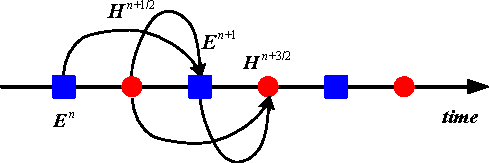
\includegraphics[width=0.7\textwidth]{L3/f1.pdf}
%\caption{\justifying{SPP的场分布}}
%\label{f1}
%\end{figure}
%\justifying{\setlength{\parindent}{2em}{因此,我们令\fcolorbox{red}{white}{$\boldsymbol{E}(x,y,z)=\boldsymbol{E}(z)\text{exp}(i\beta x),\beta=k_x$},其中$\beta$为传播常数,即$x$方向的波数$k_x$,代入亥姆霍兹方程,可得:}
%\[
%\dfrac{\partial^2\boldsymbol{E}(z)}{\partial z^2}+(k_0^2\varepsilon-\beta^2)\boldsymbol{E}(x,y,z)=0
%\]
%
%\justifying{\setlength{\parindent}{0em}{由于SPP波要在$z$方向衰减,因此需满足\fcolorbox{red}{white}{$k_0^2\varepsilon-\beta^2<0$},令$(ik_z)^2=k_0^2\varepsilon-\beta^2$,即$k_z^2-\beta^2+k_0^2\varepsilon=0$,此时方程化为了:}
%\[
%\dfrac{\partial^2\boldsymbol{E}}{\partial z^2}-k_z^2\boldsymbol{E}=0
%\]
%其解为:$\boldsymbol{E}=\boldsymbol{E}_0\text{exp}(\pm k_zz)$。
%
%\justifying{\setlength{\parindent}{2em}{综上,根据求解Maxwell方程,我们得到了电磁波沿$x$方向传播,场量与$y$无关,且在$z=0$两侧衰减的电磁场基本表达式为:}
%\[
%\boldsymbol{E}(x,z)=\boldsymbol{A_1}e^{\pm k_zz}e^{i\beta x}e^{-i\omega t}
%\]
%\[
%\boldsymbol{H}(x,z)=\boldsymbol{A_2}e^{\pm k_zz}e^{i\beta x}e^{-i\omega t}
%\]
%这里需要注意的是,$k_z$本身大于0,正负号的选择取决于介质层,若$z>0$,则取$(-)$号;若$z<0$,则取$(+)$号。
%
%\justifying{\setlength{\parindent}{2em}{知道SPP的电磁场分布基本解后,我们需要根据边界条件求SPP的色散关系。同样地,假设电流密度$\boldsymbol{J}_{\text{ext}}$为0,将本构关系$\boldsymbol{H}=\boldsymbol{B}/\mu_0$和$\nicefrac{\partial}{\partial t}=-i\omega$代入Maxwell方程组中的法拉第定律和安培-麦克斯韦定律中,可得:}
%\begin{align*}
%(1)\left\{
%\begin{array}{l}  
%  \dfrac{\partial E_z}{\partial y}-\dfrac{\partial E_y}{\partial z}=i\omega\mu_0H_x \vspace{1ex} \\ 
%  \dfrac{\partial E_x}{\partial z}-\dfrac{\partial E_z}{\partial x}=i\omega\mu_0H_y \vspace{1ex} \\
%  \dfrac{\partial E_y}{\partial x}-\dfrac{\partial E_x}{\partial y}=i\omega\mu_0H_z 
%\end{array} 
%\right.
%(2)\left\{
%\begin{array}{l}  
%  \dfrac{\partial H_z}{\partial y}-\dfrac{\partial H_y}{\partial z}=i\omega\varepsilon_0\varepsilon E_x \vspace{1ex} \\ 
%  \dfrac{\partial H_x}{\partial z}-\dfrac{\partial H_z}{\partial x}=i\omega\varepsilon_0\varepsilon E_y \vspace{1ex}\\
%  \dfrac{\partial H_y}{\partial x}-\dfrac{\partial H_x}{\partial y}=i\omega\varepsilon_0\varepsilon E_z 
%\end{array} 
%\right.
%\end{align*}
%将\fcolorbox{red}{white}{$\dfrac{\partial}{\partial x}=i\beta$、$\dfrac{\partial}{\partial y}=0$、$\dfrac{\partial}{\partial z}=\pm k_z$}代入上式,可得:
%\begin{align*}
%(1)\left\{
%\begin{array}{l}  
%  \textcolor[rgb]{1,0,0}{\pm k_zE_y=-i\omega\mu_0H_x} \vspace{1ex} \\ 
%  \textcolor[rgb]{0,0,1}{\pm k_zE_x-i\beta E_z=i\omega\mu_0H_y} \vspace{1ex}\\
%  \textcolor[rgb]{1,0,0}{i\beta E_y=i\omega\mu_0H_z}
%\end{array} 
%\right.
%(2)\left\{
%\begin{array}{l}  
%  \textcolor[rgb]{0,0,1}{\pm k_zH_y=i\omega\varepsilon_0\varepsilon E_x} \vspace{1ex} \\ 
%  \textcolor[rgb]{1,0,0}{\pm k_zH_x-i\beta H_z=-i\omega\varepsilon_0\varepsilon E_y} \vspace{1ex}\\
%  \textcolor[rgb]{0,0,1}{i\beta H_y=-i\omega\varepsilon_0\varepsilon E_z}
%\end{array} 
%\right.
%\end{align*}
%\justifying{\setlength{\parindent}{2em}{从上式可以看到,这六个等式可以分为两套独立的解,分别为:}
%\begin{align*}
%(\textcolor[rgb]{0,0,1}{1})\left\{
%\begin{array}{l}  
%  \textcolor[rgb]{0,0,1}{E_x=\pm k_zH_y/i\omega\varepsilon_0\varepsilon} \vspace{1ex}\\
%  \textcolor[rgb]{0,0,1}{E_z=-\beta H_y/\omega\varepsilon_0\varepsilon} \vspace{1ex} \\ 
%  \textcolor[rgb]{0,0,1}{(k_z^2-\beta^2+k_0^2\varepsilon)H_y=0}
%\end{array} 
%\right.
%(\textcolor[rgb]{1,0,0}{2})\left\{
%\begin{array}{l}  
%  \textcolor[rgb]{1,0,0}{H_z=\beta E_y/\omega\mu_0} \vspace{1ex} \\
%  \textcolor[rgb]{1,0,0}{H_x=\pm k_zE_y/(-i\omega\mu_0)} \vspace{1ex} \\
%  \textcolor[rgb]{1,0,0}{(k_z^2-\beta^2+k_0^2\varepsilon)E_y=0} 
%\end{array} 
%\right.
%\end{align*}
%这两套解分别对应着两种模式,即TM模和TE模,如图\ref{f2}所示。
%\begin{figure}[H]
%\centering
%	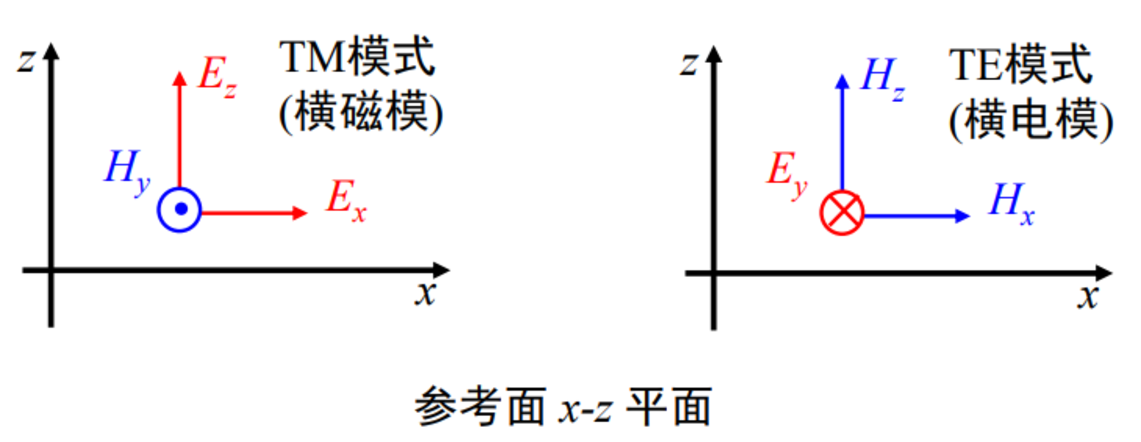
\includegraphics[width=0.7\textwidth]{L3/f2.pdf}
%\caption{\justifying{两套独立解分别代表着TM模和TE模}}
%\label{f2}
%\end{figure}
%
%\justifying{\setlength{\parindent}{2em}{先考虑TM波的情况:由于在介质1和介质2的分界面有\fcolorbox{red}{white}{$H_y$和$E_x$切向连续}这一边界条件,故对\textcolor[rgb]{0,0,1}{$\pm k_zH_y=i\omega\varepsilon_0\varepsilon E_x$}运用边界条件,可得:}
%\begin{align*}
%\left\{
%\begin{array}{l}  
%  -k_{z1}H_{y1}=i\omega\varepsilon_0\varepsilon_1E_{x1} \text{(in Medium 1)}\vspace{1ex}\\
%  k_{z2}H_{y2}=i\omega\varepsilon_0\varepsilon_2E_{x2} \text{(in Medium 2)}
%\end{array} 
%\right.
%\end{align*}
%对以上两式做比值,得到:
%\[
%\dfrac{k_{z1}}{k_{z2}}\cdot\dfrac{H_{y1}}{H_{y2}}=-\dfrac{\varepsilon_1}{\varepsilon_2}\cdot\dfrac{E_{x1}}{E_{x2}}
%\]
%化简得:
%\[
%\dfrac{k_{z1}}{k_{z2}}=-\dfrac{\varepsilon_1}{\varepsilon_2}
%\]
%若要保证$k_{z1}$和$k_{z2}$均大于零,则$\varepsilon_1$和$\varepsilon_2$必须异号,即两介质应为金属和电介质。
%
%\justifying{\setlength{\parindent}{2em}{由于$k_z^2=\beta^2-k_0^2\varepsilon$,故在不同的介质中有不同的表达式:}
%\begin{align*}
%\left\{
%\begin{array}{l}  
%  k_{z1}^2= \beta^2-k_0^2\varepsilon_1 \text{(in Medium 1)}\vspace{1ex}\\
%  k_{z2}^2= \beta^2-k_0^2\varepsilon_2 \text{(in Medium 2)}
%\end{array}   
%\right.
%\end{align*}
%联立该式($\dfrac{k_{z1}}{k_{z2}}=-\dfrac{\varepsilon_1}{\varepsilon_2}$),可以得到SPP的色散关系为:
%\[
%\beta=k_0\sqrt{\dfrac{\varepsilon_1\varepsilon_2}{\varepsilon_1+\varepsilon_2}}=\dfrac{\omega}{c}\sqrt{\dfrac{\varepsilon_m\varepsilon_d}{\varepsilon_m+\varepsilon_d}}
%\]
%\end{answer*}

\begin{problem} % 6
对于FDTD,什么是“蛙跳算法”?Yee网格有什么优势?
\end{problem}

\justifying{\setlength{\parindent}{0em}{Answer:}

\justifying{\setlength{\parindent}{2em}{在对有限差分近似公式进行离散化时,为了满足精度要求,按半步长时间交错进行$\boldsymbol{E}$和$\boldsymbol{H}$的更新,解得场的时间微分,即在时间半步长$n+1/2$处写$\boldsymbol{H}$场,在时间整步长$n$处写$\boldsymbol{E}$场,更新方程变为:}
\begin{align*}
\left\{
\begin{array}{l}  
  \boldsymbol{E}^{n+1}=\boldsymbol{E}^n+\dfrac{\Delta t}{\varepsilon}[\nabla\times\boldsymbol{H}]^{n+1/2} \vspace{1ex}\\
  \boldsymbol{H}^{n+3/2}=\boldsymbol{H}^{n+1/2}-\dfrac{\Delta t}{\mu}[\nabla\times\boldsymbol{E}]^{n+1}
\end{array} 
\right.
\end{align*}

\justifying{\setlength{\parindent}{0em}{算法示意图如下图所示:}
\begin{figure}[H]
\centering
	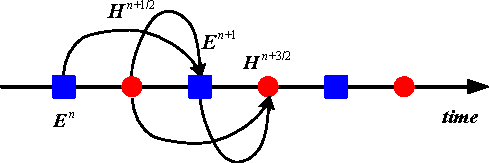
\includegraphics[width=0.7\textwidth]{L3/f1.pdf}
\caption{\justifying{蛙跳算法}}
\label{f1}
\end{figure}

\justifying{\setlength{\parindent}{2em}{Yee网格的优势有:}

\justifying{\setlength{\parindent}{0em}{1、Yee网格算法隐含地执行了两个高斯定律,同时保证了无源区域中电场和磁场都是无散的;}

\justifying{\setlength{\parindent}{0em}{2、物理边界条件($\boldsymbol{E}$和$\boldsymbol{H}$的连续性)是自然满足的;}

\justifying{\setlength{\parindent}{0em}{3、采用耦合的Maxwell旋度方程,同时在时间和空间求解电场和磁场,获得的解更加稳定;}

\justifying{\setlength{\parindent}{0em}{4、在三维空间中的各物理场分量位于不同的位置,每一个$\boldsymbol{E}$或$\boldsymbol{H}$分量由四个$\boldsymbol{H}$或$\boldsymbol{E}$循环的分量所环绕,保证了该算法同时模拟了Maxwell方程的微分形式和积分形式;}

\justifying{\setlength{\parindent}{0em}{5、即使场分量位于同一个单元内,场分量也可以在不同的材料中;}

\justifying{\setlength{\parindent}{0em}{6、场分量间不同相;}

\justifying{\setlength{\parindent}{0em}{7、与时间上的电场、磁场交叠一致。}

\begin{problem} % 7
如何由平面波展开法得到二维光子晶体的本征方程(考虑TM波)?
\end{problem}

\justifying{\setlength{\parindent}{0em}{Answer:}

\justifying{\setlength{\parindent}{2em}{平面波展开法的基本思想是,将电磁场在倒格矢空间以平面波叠加的形式展开,将麦克斯韦方程组化成一个本征方程,求解该方程的本征值便得到传播光子的本征频率。}

\justifying{\setlength{\parindent}{2em}{周期性的介电常数表示为$\varepsilon(\boldsymbol{r})=\varepsilon(\boldsymbol{r}+\boldsymbol{R})$,$\boldsymbol{R}$为晶格平移矢量,其中介电常数的倒数也是周期性的,可将其表示成一系列平面波的迭加(傅里叶级数):}
\begin{equation}
\dfrac{1}{\varepsilon(\boldsymbol{r})}=\sum_{\boldsymbol{G}}\eta_{\boldsymbol{G}}e^{\text{i}\boldsymbol{G}\cdot\boldsymbol{r}}
\label{eq7}
\end{equation}

\justifying{\setlength{\parindent}{0em}{其中$\boldsymbol{G}$是光子晶体的倒格矢,相应的傅里叶展开系数$\eta_\boldsymbol{G}$为:}
\begin{equation}
\eta_{\boldsymbol{G}}=\dfrac{1}{\Omega}\int\limits_{\text{wsc}}\dfrac{1}{\varepsilon(\boldsymbol{r})}\times e^{-\text{i}\boldsymbol{G}\cdot\boldsymbol{r}}\text{d}\boldsymbol{r}
\label{eq8}
\end{equation}

\justifying{\setlength{\parindent}{2em}{以TM模式为例,二维光子晶体中TM模电磁波的电矢量都平行于介电柱的方向(即对应的电矢量与坐标$z$无关),因此有:}
\begin{equation}
\dfrac{1}{\varepsilon(\boldsymbol{r})}\nabla^2\boldsymbol{E}(\boldsymbol{r})+\dfrac{\omega^2}{c^2}\boldsymbol{E}(\boldsymbol{r})=0
\label{eq9}
\end{equation}

\justifying{\setlength{\parindent}{0em}{由于电矢量与坐标$z$无关,故有:}
\begin{equation}
\dfrac{1}{\varepsilon(\boldsymbol{r})}(\dfrac{\partial^2}{\partial x^2}+\dfrac{\partial^2}{\partial y^2})\boldsymbol{E}_z(\boldsymbol{r})=-\dfrac{\omega^2}{c^2}\boldsymbol{E}_z(\boldsymbol{r})
\label{eq10}
\end{equation}

\justifying{\setlength{\parindent}{2em}{根据Bloch定理,电场分量可以表示成一系列平面波的迭加。将下式}
\begin{equation}
\boldsymbol{E}_z(\boldsymbol{r})=\sum_{\boldsymbol{G}}\boldsymbol{E}_{z,\boldsymbol{G}}e^{\text{i}(\boldsymbol{k}+\boldsymbol{G})\cdot\boldsymbol{r}}
\label{eq11}
\end{equation}

\justifying{\setlength{\parindent}{0em}{和级数形式(\ref{eq7})代入式(\ref{eq10}),进行适当的空间积分和代换,得到矩阵形式的本征方程:}
\begin{equation}
\sum_{\boldsymbol{G'}}\eta(\boldsymbol{G}-\boldsymbol{G'})|\boldsymbol{k}+\boldsymbol{G'}||\boldsymbol{k}+\boldsymbol{G}|\times\boldsymbol{E}_{z,\boldsymbol{G'}}=\dfrac{\omega^2}{c^2}\boldsymbol{E}_{z,\boldsymbol{G'}}
\label{eq12}
\end{equation}


\begin{problem} % 8
自然界中哪些现象与光子晶体相关,试举两个例子?
\end{problem}

\justifying{\setlength{\parindent}{0em}{Answer:}

\justifying{\setlength{\parindent}{2em}{自然界与光子晶体相关的有:蝴蝶的翅膀、变色龙的变色机理、象鼻虫外壳结构和孔雀羽毛结构等。}


\begin{problem} % 9
光子晶体带隙的物理起源是什么?三维光子晶体,哪些结构最有希望产生完全光子带隙?要获得全向带隙,除了晶体结构以外,还希望哪个参数大?
\end{problem}

\justifying{\setlength{\parindent}{0em}{Answer:}

\justifying{\setlength{\parindent}{2em}{光子带隙的物理起源是入射光频率满足布拉格条件($e^{\text{i}2ka}=1,k=\pi/a$),此时所有反射波叠加之后的反射率$R=1$(仅考虑入射光有反射),光波不能在晶体中传播,故产生了光子带隙。}

\justifying{\setlength{\parindent}{2em}{面心立方(fcc)结构是产生光子带隙最理想的结构,目前最有希望产生完全光子带隙的是fcc,金刚石和木堆积结构。}

\justifying{\setlength{\parindent}{2em}{要获得全向带隙,除了晶体结构以外,还希望光子晶体的折射率差越大越好。}



\begin{problem} % 10
为什么相对介电常数和磁导率都为负,材料的折射率为负?
\end{problem}

\justifying{\setlength{\parindent}{0em}{Answer:}

\justifying{\setlength{\parindent}{2em}{光在任何非理想材料中传输都有损耗,假设介电常数和磁导率满足:}
\begin{equation}
\varepsilon=\varepsilon_r+\text{i}\delta_1,\mu=\mu_r+\text{i}\delta_2
\label{eq13}
\end{equation}

\justifying{\setlength{\parindent}{0em}{假定损耗很小,即$\delta_i$为小量,则有:}
\begin{equation}
n^2=\varepsilon\mu\approx\varepsilon_r\mu_r+\text{i}(\varepsilon_r\delta_2+\mu_r\delta_1)
\label{eq14}
\end{equation}

\justifying{\setlength{\parindent}{0em}{若$\varepsilon_r<0$,$\mu_r<0$,根据式(\ref{eq14})可得:}
\begin{equation}
n=\pm\sqrt{\varepsilon_r\mu_r}[1-\text{i}\dfrac{(|\varepsilon_r|\delta_2+|\mu_r|\delta_1)}{2\varepsilon_r\mu_r}]
\label{eq15}
\end{equation}

\justifying{\setlength{\parindent}{0em}{介质必然是损耗介质,故折射率虚部应该大于0,因此可得:}
\begin{equation}
n=-\sqrt{\varepsilon_r\mu_r}+\text{i}\dfrac{(|\varepsilon_r|\delta_2+|\mu_r|\delta_1)}{2\sqrt{\varepsilon_r\mu_r}}
\label{eq16}
\end{equation}

\justifying{\setlength{\parindent}{0em}{此时,$n_r=-\sqrt{\varepsilon_r\mu_r}<0$,因此如果相对介电常数和磁导率都为负,材料的折射率为负。}

\begin{problem} % 11
试推导使折射率为负的必要条件。
\end{problem}

\justifying{\setlength{\parindent}{0em}{Answer:}

\justifying{\setlength{\parindent}{2em}{假设$n=n_r+\text{i}n_i$,故有:}
\begin{equation}
n^2=n_r^2-n_i^2+2\text{i}n_rn_i
\label{eq17}
\end{equation}

\justifying{\setlength{\parindent}{2em}{假设$\varepsilon=\varepsilon_r+\text{i}\varepsilon_i,\mu=\mu_r+\text{i}\mu_i$,故有:}
\begin{equation}
\varepsilon\mu=(\varepsilon_r+\text{i}\varepsilon_i)(\mu_r+\text{i}\mu_i)=(\varepsilon_r\mu_r-\varepsilon_i\mu_i)+\text{i}(\varepsilon_r\mu_i+\varepsilon_i\mu_r)
\label{eq18}
\end{equation}

\justifying{\setlength{\parindent}{0em}{由于$n^2=\varepsilon\mu$,故对应虚部相等,即:}
\begin{equation}
2n_rn_i=\varepsilon_r\mu_i+\varepsilon_i\mu_r
\label{eq19}
\end{equation}

\justifying{\setlength{\parindent}{0em}{因为$n_i>0$,故若使$n_r<0$,则只需$\varepsilon_r\mu_i+\varepsilon_i\mu_r<0$即可,此即为使折射率为负的必要条件。}














%\begin{problem}
%
%Consider the following decision rule for a two-category one-dimensional problem: 
%Decide \(\omega_1\) if \(x > \theta\); otherwise decide \(\omega_2\).
%
%(a) Show the probability of error for this rule is given by
%\[
%P(\text{error}) = P\left(\omega_{1}\right) \int_{-\infty}^{\theta} p\left(x | \omega_{1}\right) \mathrm{d}x+P\left(\omega_{2}\right) \int_{\theta}^{\infty} p\left(x | \omega_{2}\right) \mathrm{d}x.
%\]
%
%(b) By differentiating, show that a necessary condition to minimize \(P(\text{error})\) is that satisfy
%\[
%p(\theta | \omega_1) P(\omega_1) = p(\theta | \omega_2) P(\omega_2).
%\]
%
%(c) Does this equation define \(\theta\) uniquely?
%
%(d) Give an example where a value of \(\theta\) satisfying the equation actually maximizes the probability of error.
%
%\end{problem}
%
%\begin{answer}
%考虑分类错误率的条件概率:
%\begin{equation}
%	P(\text{error} | x) =
%	\begin{cases}
%		p(\omega_1 | x), & \text{if we decide }\omega_2, \\
%		p(\omega_2 | x), & \text{otherwise.}
%	\end{cases}
%	\label{eq:error-conditional-probability}
%\end{equation}
%
%根据式 (\ref{eq:error-conditional-probability}) 对\(x\)进行积分,可得:
%\begin{align}
%	P(\text{error}) & = \int_{-\infty}^\infty P(\text{error} | x) p(x) \mathrm{d} x \\
%	& = P(x \leq \theta , x \text{ is } \omega_1 ) + P(x > \theta , x \text{ is } \omega_2 ) \\
%	& = p(x \leq \theta | \omega_1) P(\omega_1) + p(x > \theta | \omega_2) P(\omega_2) \\
%	& = P\left(\omega_{1}\right) \int_{-\infty}^{\theta} p\left(x | \omega_{1}\right) \mathrm{d} x + P\left(\omega_{2}\right) \int_{\theta}^{\infty} p\left(x | \omega_{2}\right) \mathrm{d} x. \label{eq:error-probability}
%\end{align}
%\end{answer}
%
%\makecomputerexercise
%
%Several of the computer exercises will rely on the following data.
%
%此处还可以插入一些说明。
%
%\begin{computerexercise}
%Illustrate the fact that the average of a large number of independent random variables will approximate a Gaussian by the following:
%
%(a) Write a program to generate n random integers from a uniform distribution \(U(x_l, x_u)\).
%
%(b) Now write a routine to choose \(x_l\) and \(x_u\) randomly, in the range \(-100 \leq x_l < x_u \leq 100\), and \(n\) (the number of samples) randomly in the range \(0 < n \leq 1000\).
%
%(c) Generate and plot a histogram of the accumulation of \(10^4\) points sampled as just described.
%
%(d) Calculate the mean and standard deviation of your histogram, and plot it.
%
%(e) Repeat the above for \(10^5\) and for \(10^6\). Discuss your results.
%\end{computerexercise}
%
%\begin{answer}
%答案写在此处,如代码~\ref{lst:python}~所示。
%
%\begin{lstlisting}[language=python,caption=代码测试,label=lst:python]
%print('Hello, world!')
%\end{lstlisting}
%
%为了得到\(p(x | \omega) \sim \mathcal{N}(0, 1)\):
%\begin{equation}
%	p(x | \omega_i) = \frac{1}{\sqrt{2 \pi} \sigma}\exp{\left[- \frac{1}{2} \left(\frac{x - \mu}{\sigma}\right)^2\right]}
%	\label{eq:Gaussian-distribution}
%\end{equation}
%
%对式 (\ref{eq:Gaussian-distribution}),我们可以进行一些计算。
%
%\end{answer}
%
%%% 插入matlab代码
%\lstinputlisting[style=Matlab-editor,basicstyle=\mlttfamily,numbers=left,frame=single,caption={\bf main.m}]{L3/sample.m}
%%% 插入表格
%\begin{table}
%    \centering
%    \fontsize{8}{10}\selectfont    %{字体尺寸}{行距}
%    \caption{工作原理}
%	\begin{tblr}{
%        row{odd} = {bg=azure8},
%        row{1} = {bg=azure3, fg=white},
%        colspec={c|ccc},
%        }
%	    \toprule
%		\diagboxthree{偏振方向}{属性}{位置/晶向} & \mbox{左($\updownarrow$)} & \mbox{右($\odot$)} & \mbox{偏折} \\
%	    \specialrule{0.5pt}{4pt}{6pt}
%		$\updownarrow$ & \mbox{$e$($n$小)} & \mbox{$o$($n$大)} & \mbox{靠近法线}\\
%		$\odot$ & \mbox{$o$($n$大)} & \mbox{$e$($n$小)} & \mbox{远离法线}\\
%	    \bottomrule 
%	\end{tblr}
%    \label{tab:Training_sizes}
%\end{table}
%%% 插入图片
%\begin{figure}[H]
%\centering
%	\includegraphics[width=0.9\textwidth]{L3/Fig3_5.pdf}
%\caption{\justifying{Orientation of $\boldsymbol{E}$ vector at various locations along the $z$-axis.}}
%\label{f3_5}
%\end{figure}
%%% 首行缩进
%\justifying{\noindent 即此式也为直线方程,即出射光仍为线偏振光,只是振动面的方位较入射光即此式也为直线方程,即出射光仍为线偏振光,只是振动面的方位较入射光}
%
%\justifying{\setlength{\parindent}{2em} 即此式也为直线方程,即出射光仍为线偏振光,只是振动面的方位较入射光即此式也为直线方程,即出射光仍为线偏振光,只是振动面的方位较入射光}
%
%%% 引用参考文献
%\justifying{\noindent 显然,此式为直线方程,即线偏振光通过全波片后,其偏振状态不变。这里还有另一种理解方式\citep{ref3_1},现在,$\vv{a}$我们\fcolorbox{white}{green}{\mbox{我们}}考虑具有相同振幅的且具有相同相位(或相位差为$2\pi$整数倍)的两个波,在这里我们只考虑线偏振情况。}
%
%% 参考文献
%
%\begin{thebibliography}{23}
%
%\bibitem{ref3_1} %1
%Ashim Kumar Bain, ``Crystal Optics: Properties and Applications'', \sourcelink{10.1002/9783527823017}{Wiley Online} , Online ISBN: \textbf{9783527823017}(2019).
%
%\end{thebibliography}
\end{document}
